\documentclass[11pt]{article}

% Libraries.
\usepackage{amsmath}
\usepackage{amssymb}
\usepackage{pgfplots}
\usepackage{graphicx}
\usepackage{enumitem}
\usepackage{hyperref}
\usepackage{fancyhdr}
\usepackage{perpage}
\usepackage{float}
\usepackage{graphicx}
\graphicspath{ {./images/} }

% Property settings.
\MakePerPage{footnote}
\pagestyle{fancy}
\lhead{Notes by Y.W.}

% Commands
\newcommand{\ti}[1]{\textit{#1}}
\newcommand{\tb}[1]{\textbf{#1}}
\newcommand{\mb}[1]{\mathbb{#1}}
\newcommand{\under}[1]{\underline{#1}}
\newcommand{\proof}[0]{\textit{\underline{proof:} }}
\newcommand{\litran}[0]{$T: V \rightarrow W$ }
\newcommand{\slitran}[0]{Let $ T: V \rightarrow W$ be a linear transformation }
\newcommand{\mt}[0]{$[T]_\alpha^\beta$ }
\newcommand{\qed}[0]{$\hfill\blacksquare$}
\newcommand{\real}[0]{\mathbb{R}}
\newcommand{\vx}[0]{\tb{x}}
\newcommand{\vy}[0]{\tb{y}}
\newcommand{\vz}[0]{\tb{z}}
\newcommand{\vo}[0]{\tb{0}}
\newcommand{\vu}[0]{\tb{u}}
\newcommand{\vw}[0]{\tb{w}}
\newcommand{\vv}[0]{\tb{v}}
\newcommand{\vf}[0]{\tb{f}}
\newcommand{\vm}[0]{\tb{m}}
\newcommand{\trans}[3]{{#1}: {#2} \rightarrow {#3}}

% Attr.
\title{Advanced Math Notes}
\author{Yuchen Wang}
\date{\today}

\begin{document}
	\maketitle
	\tableofcontents
	\newpage
	\section{Free parameter}
	A variable in a mathematical model which cannot be predicted precisely or constrained by the model and must be estimated experimentally or theoretically.
	\section{Rectifier}
	\subsection{Definition}
	An activation function defined as the positive part of its argument:
	$$f(x) = \max(0,x)$$
	Also known as: ramp function \\
	A unit employing the rectifier is also called a \tb{rectified linear unit (ReLU)}
	\subsection{Softplus}
	A smooth approximation to the rectifier is the analytic function $$f(x) = \log(1+e^x)$$
	Also known as: SmoothReLU\\
	The derivative of softplus is $$f'(x) = \frac{1}{1+e^{-x}}$$(the logistic function)
	\paragraph{Notes}
	The logistic function is a smooth approximation of the derivative of the rectifier, the \tb{Heaviside step function}
	\subsection{Multivariable Generalization to Softplus}
	LogSumExp with the first argument set to zero
	$$LSE_0^+(x_1,\hdots,x_n) := LSE(0,x_1,\hdots,x_n) = \log(1+e^{x_1} + \hdots + e^{x_n})$$
	\paragraph{Notes}
	The LogSumExp function itself is:
	$$LSE(x_1,\hdots,x_n) = \log(e^{x_1} + \hdots + e^{x_n})$$
	and its gradient is the softmax.\\
	The softmax with the first argument set to zero is the multivariable generalization of the logistic function.
	\section{Softmax Function}
	The softmax function takes an un-normalized vector, and normalizes it into a probability distribution. That is, prior to applying softmax, some vector elements could be negative, or greater than one; and might not sum to 1; but after applying softmax, each element $x_i$ is in the interval $[0,1]$, and $\sum_i x_i = 1$ \\
	$$\sigma:\real^K \rightarrow \{\sigma\in \real^K|\sigma_i>0,\sum_{i=1}^K \sigma_i = 1\}$$
	$$\sigma(\vz)_j = \frac{e^{z_j}}{\sum_{k=1}^K e^{z_k}}$$ for $j = 1,\hdots,K$
	
	\section{Cross Entropy}
	The \under{Cross entropy} between two probability distributions $p$ and $q$ over the same underlying set of events measures the average number of bits needed to identify an even drawn from the set if a coding scheme used for the set is optimized for an estimated probability distribution $q$, rather than the true distribution $p$.
	\paragraph{Discrete distributions}
	$$ H(p, q) = - \sum_{x \in \chi} p(x) \, \log q(x) $$
	\paragraph{Continuous distributions}
	$$ H(p, q) = - \int_\chi P(x)\, \log Q(x) \, dr(x) $$
	\section{Cross Product in Higher Dimensions}
	A way of turning 3 vectors in 4-space into a fourth vector, orthogonal to the others, in a trilinear way \\
	Canonical basis of $\real^4: (e_1, e_2, e_3, e_4)$. If your vectors are $\tb{t} = (t_1, t_2, t_3, t_4), \tb{u} = (u_1, u_2, u_3, u_4)$ and $\tb{v} = (v_1, v_2, v_3, v_4)$, then compute the determinant:
	$$\begin{vmatrix}
	t_1 & t_2 & t_3 & t_4 \\
	u_1 & u_2 & u_3 & u_4 \\
	v_1 & v_2 & v_3 & v_4 \\
	e_1 & e_2 & e_3 & e_4
	\end{vmatrix}$$
	The cross product of $\tb{t}, \tb{u}, \tb{v}$ is:
		$$-e_1\begin{vmatrix}
	 t_2 & t_3 & t_4 \\
	 u_2 & u_3 & u_4 \\
	 v_2 & v_3 & v_4 \\
	\end{vmatrix}
	+e_2\begin{vmatrix}
	t_1 & t_3 & t_4 \\
	u_1 & u_3 & u_4 \\
	v_1 & v_3 & v_4 \\
	\end{vmatrix}
	- e_3\begin{vmatrix}
	t_1 & t_2 & t_4 \\
	u_1 & u_2 & u_4 \\
	v_1 & v_2 & v_4 \\
	\end{vmatrix}
	+ e_4\begin{vmatrix}
	t_1 & t_2 & t_3 \\
	u_1 & u_2 & u_3 \\
	v_1 & v_2 & v_3 \\
	\end{vmatrix}
	$$
\section{Gaussian Process}
\subsection{The Basics}
\paragraph{Definition 1}
We use a \under{Gaussian process} to describe a distribution over functions:
$$\tb{f} \sim \mathcal{GP}(m, K)$$ 
where $m: \chi \rightarrow \real$ is the \under{mean function}
$$m(\vx) = E[f(\vx)]$$
and $K: \chi^2 \rightarrow \real$ is the \under{covariance function}
$$K(\vx, \vx') = E[(f(\vx) - m(\vx))(f(\vx') - m(\vx'))]$$
\paragraph{Definition 2}
For any set $S$, a \under{Gaussian Process} on S is a set of r.v.s $Z_t: t\in S$ s.t. $\forall n \in \mathbb{N}, \forall t_1,\hdots,t_n \in S, (Z_{t_1},\hdots, Z_{t_n})$ is multi-variate Gaussian.
\paragraph{Theorem: Existence of Gaussian Process}
For any set $S$, any mean function $\mu: S \rightarrow \real$, and any covariance function $k: S\times S \rightarrow \real$, there exists a GP $Z_t$ on S s.t. $E(Z_t) = \mu(t), Cov(Z_s, Z_t) = k(s,t) \, \forall s, t\in S$.

\paragraph{GPs define multivariate Gaussian distributions}
We have data points $X = [\vx_1^T, \hdots, \vx_n^T]^T$ and are interested in their function values $\tb{f}(X) = (f(\vx_1), \hdots, f(\vx_n))^T$.\\
$\tb{f}$ is one subset of r.v. and has (prior) joint Gaussian distribution:
$$\vf(X) \sim \mathcal{N}(\vm(X),K(X,X))$$
\paragraph{Remarks}
\begin{enumerate}
	\item The covariance function $K(\vx, \vx')$ returns a measure of the similarity of $\vx$ and $\vx'$ that also encodes how similar $f(\vx)$ and $f(\vx')$ should be.
	\item The mean function $m(\vx)$ encodes a prior expectation of the (unknown) function
\end{enumerate}

\paragraph{Setting the mean function}
In most cases we simply use
$$E(f(\vx)) = m(\vx) = 0$$
which makes sense especially if we normalize the output to zero mean.
\paragraph{Properties of the covariance function}
The covariance function $K(\vx,\vx')$ needs to be a measure of similarity between $\vx$ and $\vx'$.
\begin{enumerate}
	\item K needs to be symmetric $$K(\vx, \vx') = K(\vx', \vx)$$
	\item K needs to be positive semidefinite (nonnegative definite) $$\int_{-\infty}^\infty\int_{-\infty}^{\infty} K(\vx, \vx')g(\vx)g(\vx')\,d\vx d\vx' \geq 0$$ for all $g \in L_2$.
\end{enumerate}

\paragraph{Setting the covariance function}
\begin{enumerate}
	\item \under{Gaussian Kernel}:
$$K(r) = \theta_A^2 \exp[-\frac{r^2}{2\theta_L^2}]$$
\item \under{Periodic Covariance Function}
$$K(r) = \theta_A^2\exp[-\frac{\sin^2[(2\pi/\theta_P)r]}{2}]$$
where $r = ||x-x'||$ denotes the Euclidean distance between two indexes.
\end{enumerate}
\paragraph{Hyperparameters}
$\theta_A$:  $y$-scaling \\
$\theta_L$:  $x$-scaling (or time scale if the data are time series) \\
$\theta_P$:  period of the covariance functions \\
\subsection{Gaussian Process Regression}
Basically equivalent to Bayesian linear regression.\\
Twist is that using kernel instead of basis functions in order to define the family of functions that you are using for regression.\\
This allows us to define a very rich family of functions that using basis functions alone could not handle (e.g. mapping into an infinite dimensional space).\\
In a Gaussian Process regression model, mathematically the same inference as in linear regression can be done.
\paragraph{The model}
Let $Z \in \real^n \sim N(\mu, K), \varepsilon \in \real^n \sim N(0, \sigma^2I)$ be independent r.v.s. Let $y = Z + \varepsilon$, so $y \sim N(\mu, K+\sigma^2I)$.\\
Define $C = K + \sigma^2 I$.\\
Let $a = (1, \hdots, l), b = (l+1, \hdots, n)$, so $y = \begin{pmatrix}
	y_a \\ y_b \end{pmatrix}$, where $y_a = \begin{pmatrix} y_1 \\ \vdots \\y_l
	\end{pmatrix}, y_b = \begin{pmatrix} y_{l+1} \\ \vdots \\ y_n \end{pmatrix}$.
	In addition, $\mu = \begin{pmatrix} \mu_a \\ \mu_b \end{pmatrix}, C = \begin{pmatrix} C_{aa} & C_{ab} \\ C_{ba} & C_{bb} \end{pmatrix}, K = \begin{pmatrix} K_{aa} & K_{ab} \\ K_{ba} & K_{bb} \end{pmatrix}$\\
Then we have $(Y_a | Y_b = y_b) \sim N(m, D)$, where 
\begin{align*}
	m &= \mu_a + C_{ab}C^{-1}_{bb}(y_b - \mu_b) \\
	&= \mu_a +K_{ab}(K_{bb} + \sigma^2 I)^{-1}(y_b - \mu_b)\\
	D &= C_{aa} - C_{ab}C^{-1}_{bb}C_{ba} \\
	&= (K_{aa}+\sigma^2 I)-K_{ab}(K_{bb}+\sigma^2I)^{-1}K_{ba}
\end{align*}
\paragraph{Parameters}
\begin{enumerate}
	\item $\mu$
	\item $K$
\end{enumerate}
\paragraph{Inference}
\begin{enumerate}
	\item Plot the mean function to predict unobserved values (good for visualization)
	\item Plot the error curves
	\item Choose a loss function and minimize the loss using posterior distribution
\end{enumerate}
\paragraph{Negative Log Marginal Likelihood (NLML)}
The values of hyperparameters $\theta$ may be optimized by minimizing NLML:
\begin{align*}
	NLML &= -\log p(\vy|\vx,\theta) \\
	&= \frac{1}{2}\log |K| + \frac{1}{2}\vy^TK^{-1}\vy + \frac{n}{2} \log (2\pi)
\end{align*}
\section{Kronecker Product}
A generalization of the outer product from vectors to matrices.
\paragraph{Definition}
$$A \otimes B = \begin{bmatrix}
	a_{11}B & \hdots & a_{1n}B \\
	\vdots & \ddots & \vdots \\
	a_{m1}B & \hdots & a_{mn}B
\end{bmatrix}$$
\section{Bayes' Theorem}
$$P(A|B) = \frac{P(B|A)P(A)}{P(B)}$$
where $A$ and $B$ are events and $P(B) \neq 0$.
\section{Maximum a Posteriori Estimation (MAP)}
An estimate of an unknown quantity that equals the mode of the posterior distribution. \\
Can be used to obtain a \textcolor{blue}{point estimate} of an unobserved quantity on the basis of empirical data.\\
Closely related to MLE but employs an augmented optimization objective which incorporates a prior distribution (fix the overfitting problem). \\
Can be seen as a regularization of MLE.
\paragraph{Description}
Assume we want to estimate an unobserved population parameter $\theta$ on the basis of observations $x$> Let $f$ be the sampling distribution of $x$ so that $f(x|\theta)$ is the probability of $x$ when the underlying population parameter is $\theta$. \\
Now assume that a prior distribution $g$ exists. This allows us to treat $\theta$ as a random variable. By Bayes' Theorem, the posterior distribution of $\theta$ is 
$$f(\theta|x) = \frac{f(x|\theta)g(\theta)}{\int_\Theta f(x|v)g(v)\,dv}$$
where $g$ is the density function of $\theta$, $\Theta$ is the domain of $g$.
Then
$$\hat{\theta}_{MAP}(x) = \underset{\theta}{argmax} f(\theta|x)$$
\section{Bayesian Linear Regression}
Why not use MLE? - overfitting \\
Why not use MAP? - no representation of uncertainty
\paragraph{Setup}
$$D = ((x_1, y_1), \hdots, (x_n, y_n)), x_i \in \real^d, y_i \in \real$$
\paragraph{Model}
$y_1, \hdots, y_n$ indep given $w$, $y_i \sim N(w^Tx_i, a^{-1}), a>0$ \\
$w \sim N(0,b^{-1}I), b>0. \, (w=(w_1,\hdots,w_d))$ \\
($a, b:= 1/ variance$ is called precision) \\
Assume $a,b$ are known so the only parameter is $w$.
\paragraph{Posterior Distribution of $w$}
It can be shown that $$P(w|D) = N(w|\mu, \Lambda^{-1})$$
where $\mu = a\Lambda^{-1}X^Ty$ and $\Lambda = aX^TX+bI$ where $X$ is the design matrix.
\section{Laplace Distribution}
Sometimes also called "double exponential distribution", because it can be though of as two exponential distributions (with an additional location parameter) spliced together back-to-back.
\paragraph{PDF}
$$\frac{1}{2b}\exp(-\frac{|x-\mu|}{b}$$
\begin{figure}[h]
	\centering
	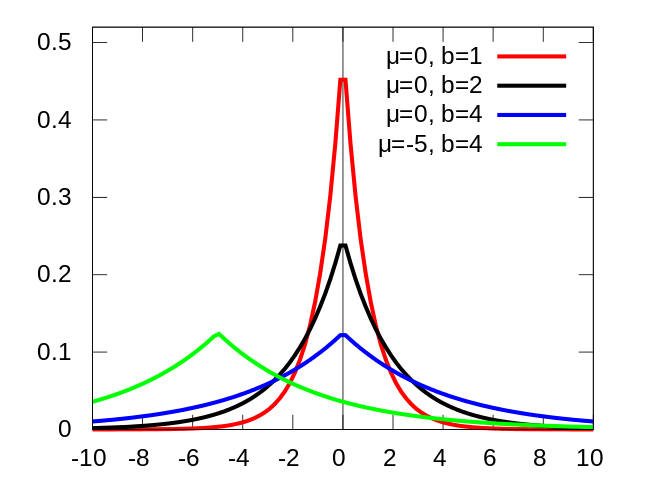
\includegraphics[scale=0.3]{laplace.png}
	\caption{PDF of Laplace Distribution}
\end{figure}

\section{Kullback-Leibler Divergence}
Also called ``relative entropy", is a measure of how one probability distribution is different from a second, reference probability distribution.
\paragraph{Definition}
For discrete probability distribution $P$ and $Q$ defined on the same probability space, the \under{Kullback-Leibler divergence} between $P$ and $Q$ is defined to be
$$D_{KL}(P|Q) = - \sum_{x \in \chi} P(x)\log(\frac{Q(x)}{P(x)})$$
For distributions $P$ and $Q$ of a continuous random variable, the Kullback-Leiber divergence is defined to be the integral
$$D_{KL}(P|Q) = \int_{-\infty}^\infty p(x)\log(\frac{p(x)}{q(x)})\, dx$$ where $p$ and $q$ denote the probability densities of $P$ and $Q$.

 
\end{document}
